\section{Development}
\subsection{Methods}

The additions that need to be made to the GNSS-SDR framework to implement the robust Kalman filter-based carrier synchronization proposed in this document are twofold: First, software for performing carrier synchronization using a Kalman filter-based approach will need to be developed based on standard filter algorithms without robust covariance estimation. Currently, the GNSS-SDR project performs carrier synchronization using a digital DLL/PLL-based architecture, so implementation of even standard filter methodology will involve the development of an entirely new architecture and parallel data pathway for the carrier synchronization portion of the receiver. It is believed that development, integration and testing of the architecture based on the standard Kalman methodology within the GNSS-SDR framework will represent the bulk of effort required for this contribution. Second, once the Kalman filter-based approach is implemented using standard Kalman filter methodology, that software can then be modified to perform robust covariance estimation. This should not be as significant a body of effort as the development of the basic Kalman architecture, but as it constitutes a departure from the established Kalman techniques for performing phase estimation, it will require additional prototyping and performance testing that would not be of as much value for the traditional Kalman methods.

\subsection{Timeline}

We anticipate that some of the prototyping work for the robust covariance estimation methods (e.g. in MATLAB) can be performed in parallel with the development of the Kalman filter architecture within the GNSS-SDR framework. Based on the Phase 1-3 breakdown provided by the Google Summer of Code program, we propose the following goals:

\textbf{Phase 1}, 14-May-2018 to 15-June-2018: Development and integration of standard Kalman filter based methodology into the carrier synchronization portion of the GNSS-SDR datapath. Both discriminator-based and discriminator-free architectures will be considered here. Preliminary results from prototyping the covariance estimation methods.

\textbf{Phase 2}, 15-June-2018 to 13-July-2018: Testing of standard Kalman filter based methodology into the carrier synchronization portion of the GNSS-SDR datapath, and final results from prototyping the covariance estimation methods.

\textbf{Phase 3}, 13-July-2018 to 14-August-2018: Development and integration of robust Kalman filter based methodology with covariance estimation into the carrier synchronization portion of the GNSS-SDR datapath.





\subsection{Access to a professional GNSS signal simulator}\label{sec:intro:approach:synthdata}

\begin{wrapfigure}{R}{0.5\textwidth}
\centering
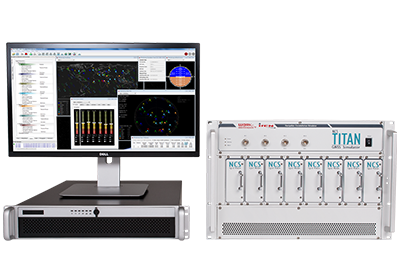
\includegraphics[width=0.48\textwidth]{fig/NCS-Titan_GNSS_Simulator.png}
%\caption{Low-cost ISM Receiver Architecture Scheme}\label{fig:Rx}
\end{wrapfigure}
As a complement, particularly useful in the design phase of the project where methods are adjusted, it is worth mentioning here that have access to a powerful GNSS signal simulator. Namely, the lab I am member of has acquired the NCS Titan GNSS Simulator, the latest product from IFEN. The Titan is a multi-GNSS, multi-frequency and multi-RF output simulator, featuring high fidelity, flexibility and scalability. The available equipment can simulate up to 256 channels and up to 2 RF outputs, generating GPS L1, GPS L5, Galileo E1, and Galileo E5 signals. Among the many characteristics of this high-grade signal simulator, it is of interest here that it is able to incorporate jamming and spoofing attacks, as well as relevant receiver imperfections. This equipment is crucial to test the developed methodologies in a controlled manner, before validation through real data. Additionally, we own USRP and HackRF front-ends which will be used to connect the GNSS Simulator with the GNSS-SDR receiver. This front-ends are a perfect example of the versatile, low-cost hardware components we are interested in this project, featuring a rather poor clock accuracy around $1$ to $20$ ppm depending on the hacks.